\chapter{Mordente}

Tras estudiar la motivación de este trabajo y habiendo justificado la necesidad de una alternativa software para la gestión de agrupaciones musicales, pasamos a desarrollar el producto. Para esta fase se va a hacer uso de la llamada metodología de Diseño Centrado en el Usuario (UCD por sus siglas en inglés), descrita en el siguiente apartado. 

\section{Desarrollo de Mordente}

En este punto se van a establecer las metodologías de diseño a seguir durante el desarrollo de la herramienta, de modo que tengamos disponibles unas guías a seguir durante el proceso y unas herramientas que nos permitan definir la funcionalidad esperada y concretar las necesidades de los futuros usuarios.

\subsection{Diseño Centrado en el Usuario}

El Diseño Centrado en el Usuario está estrechamente relacionado con el Diseño Centrado en el Humano\cite{w3UCD}. Este último ``es una aproximación al desarrollo de sistemas interactivos que se centra específicamente en hacer sistemas usables. Es una actividad multi-disciplinar.''\cite{isoHCD}.

Los principios\cite{jeffreyUCD} en los que se fundamenta se pueden resumir en:

\begin{enumerate}
    \item \textbf{Aproximación temprana a usuarios y tareas}: la recogida de información es estructurada y sistemática.
    \item \textbf{Medida empírica y testeo del uso del producto}: se centra en la facilidad de aprendizaje y de uso, y la prueba de prototipos con usuarios reales.
    \item \textbf{Diseño iterativo}: el producto se diseña, modifica y prueba de forma repetida, permitiendo repensar completamente la idea gracias a la prueba de modelos conceptuales tempranos.
\end{enumerate}

\subsection{Design Thinking}

El Design Thinking es un proceso de diseño descrito en cinco fases:\cite{designThinkingPlattner} definir el problema, buscar las necesidades, idear, construir y probar. Este proceso nos ayuda a aplicar el Diseño Centrado en el Usuario mediante una serie de procesos.

\subsubsection{Procesos}

Otros autores hablan de que el Design Thinking no se compone de fases sino de varios espacios que no son secuenciales: se solapan y se forma un bucle entre ellos, repitiéndolo más de una vez y explorando distintas aproximaciones\cite{designThinkingBrown}.

\begin{enumerate}
    \item \textbf{Inspiración}: se observa cómo funcionan las personas para encontrar problemas y oportunidades.
    \item \textbf{Empatía}: se trata de entender los deseos y necesidades de los potenciales clientes, no solo de forma técnica sino sabiendo por qué hacen las cosas de la forma actual y qué les resulta más importante.
    \item \textbf{Ideación}: se trata de una combinación de pensamiento divergente y convergente. El pensamiento divergente genera nuevas ideas de forma creativa, mientras que el convergente trata de sintetizar las ideas y elegir las mejores.
    Teniendo diversas personas en el equipo, la técnica más utilizada es el \textit{brainstorming}, en el que todos los miembros dan ideas espontáneas que se apuntan de forma que cada nueva idea puede fomentar la creatividad de los demás.
    \item \textbf{Implementación y prototipado}: en este proceso las ideas se convierten en productos concretos. Durante este proceso se van generando diversos prototipos que se prueban con usuarios reales para seguir mejorando la idea.
\end{enumerate}


\section{Personas ficticias}

Las personas ficticias se crean dentro de una técnica perteneciente al Design Thinking. Se tratan de representaciones ficticias de los usuarios, con metas, motivaciones, características y comportamientos de un grupo real de usuarios.\cite{personnas}

Esta técnica nos permite diseñar para personas reales y no para ``usuarios'' abstractos.

En el caso del proyecto que nos ocupa, se han creado cuatro personas ficticias: dos que cumplirían el rol de ``administrador'' en el sistema y otras dos que lo usarían únicamente como miembros.

\begin{figure}[h]
\centering
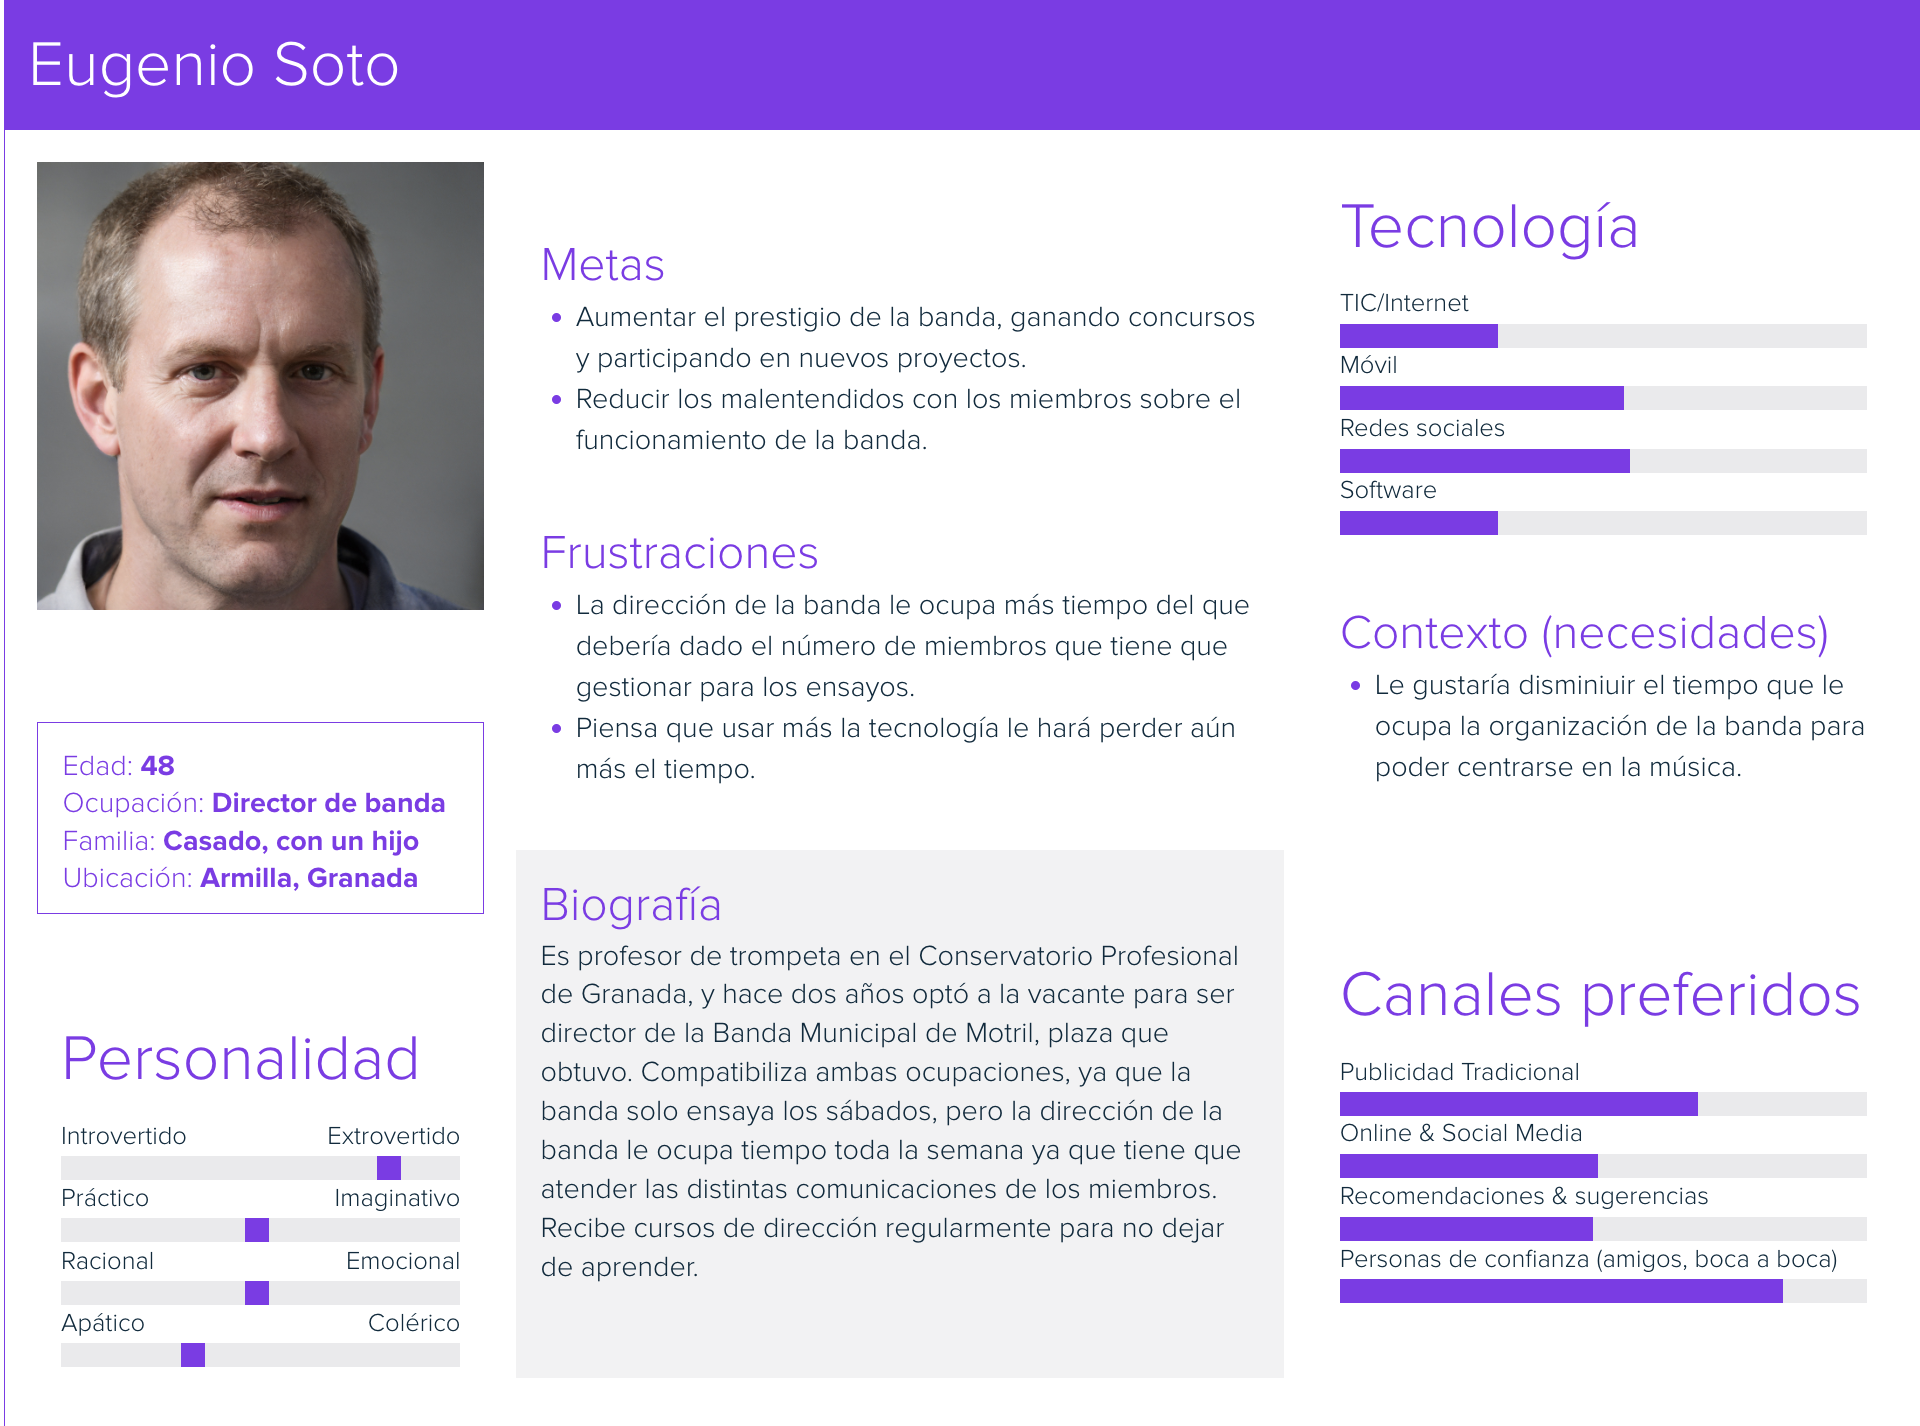
\includegraphics[width=0.8\textwidth]{imagenes/personas/persona_eugenio.png}
\caption{Persona: Eugenio Soto}
\label{fig:persona_eugenio}
\end{figure}

\begin{figure}[h]
\centering
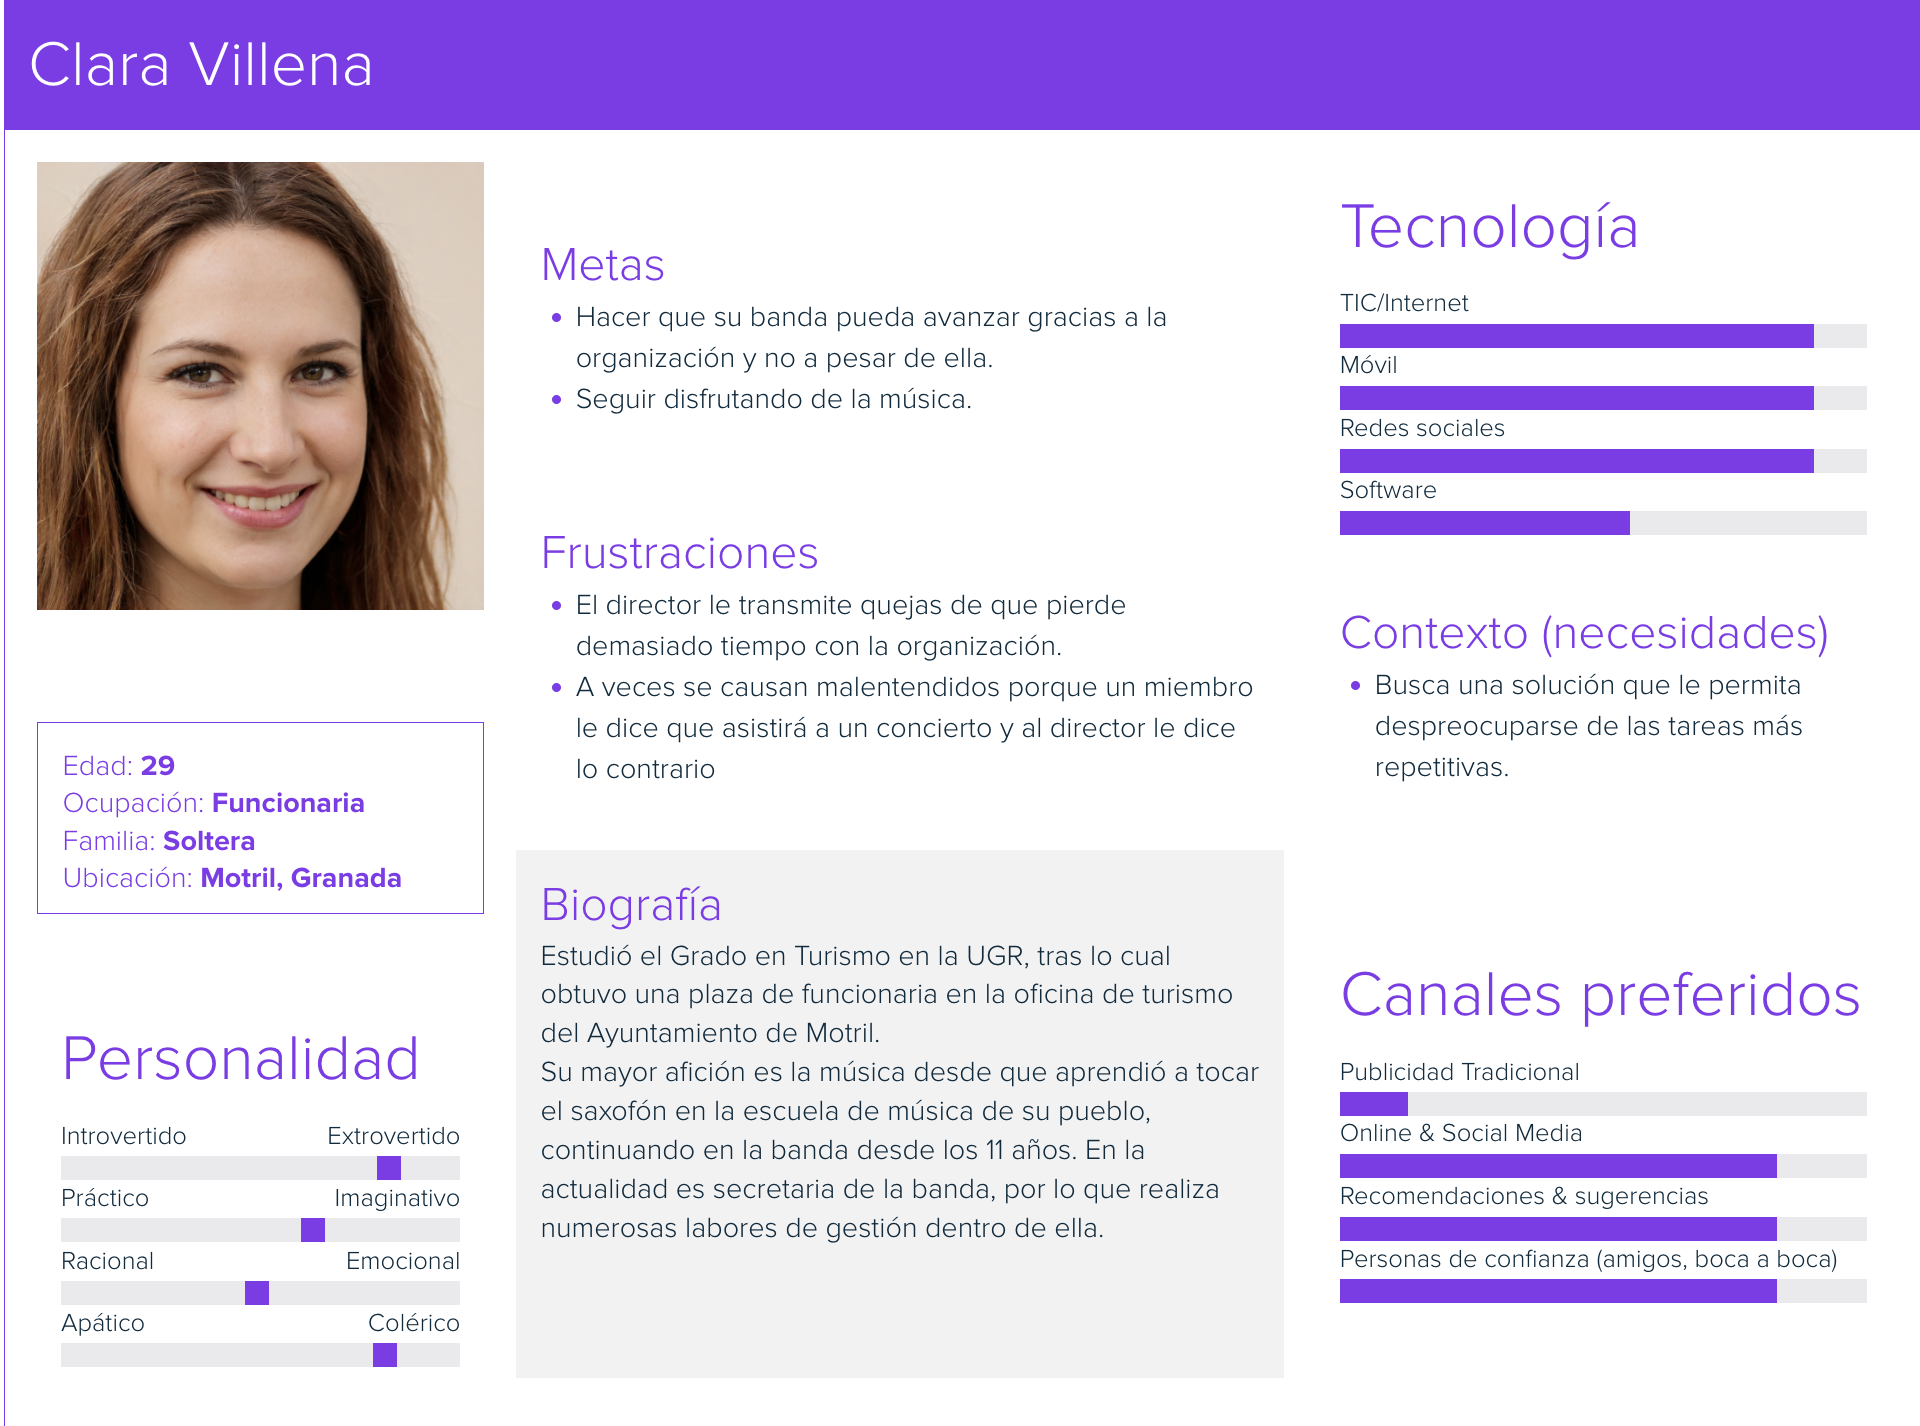
\includegraphics[width=0.8\textwidth]{imagenes/personas/persona_clara.png}
\caption{Persona: Clara Villena}
\label{fig:persona_clara}
\end{figure}


Las figuras \ref{fig:persona_eugenio} y \ref{fig:persona_clara} muestran dos personas que se dedican a la organización de la banda, Eugenio más desde el punto de vista musical y Clara desde el logístico.

Mientras Clara está claramente más familiarizada con las nuevas tecnologías, Eugenio muestra algunas reticencias que deberemos tratar durante el desarrollo, de forma que el producto final sea fácilmente usable y accesible. Igualmente, ya que Clara sí usa las nuevas tecnologías habitualmente, el producto tiene que ser atractivo para ella de forma que no suponga un retroceso con respecto a las herramientas actuales.

Los perfiles que vemos en las figuras \ref{fig:persona_david} y \ref{fig:persona_inma} se refieren a personas que acuden como miembros a la banda de su respectivo pueblo. A Inma se aplican las mismas restricciones que a Eugenio, además de que debemos asegurarnos de que realmente facilitamos que los miembros recuerden los eventos diarios para hacerles la vida más fácil. Con respecto a David, cabe reseñar que, ya que la música no es su mayor afición, preferirá usar la app durante el menor tiempo posible, por lo que se debe intentar que las notificaciones que le lleguen le permitan responder de forma rápida.



\begin{figure}[h]
\centering
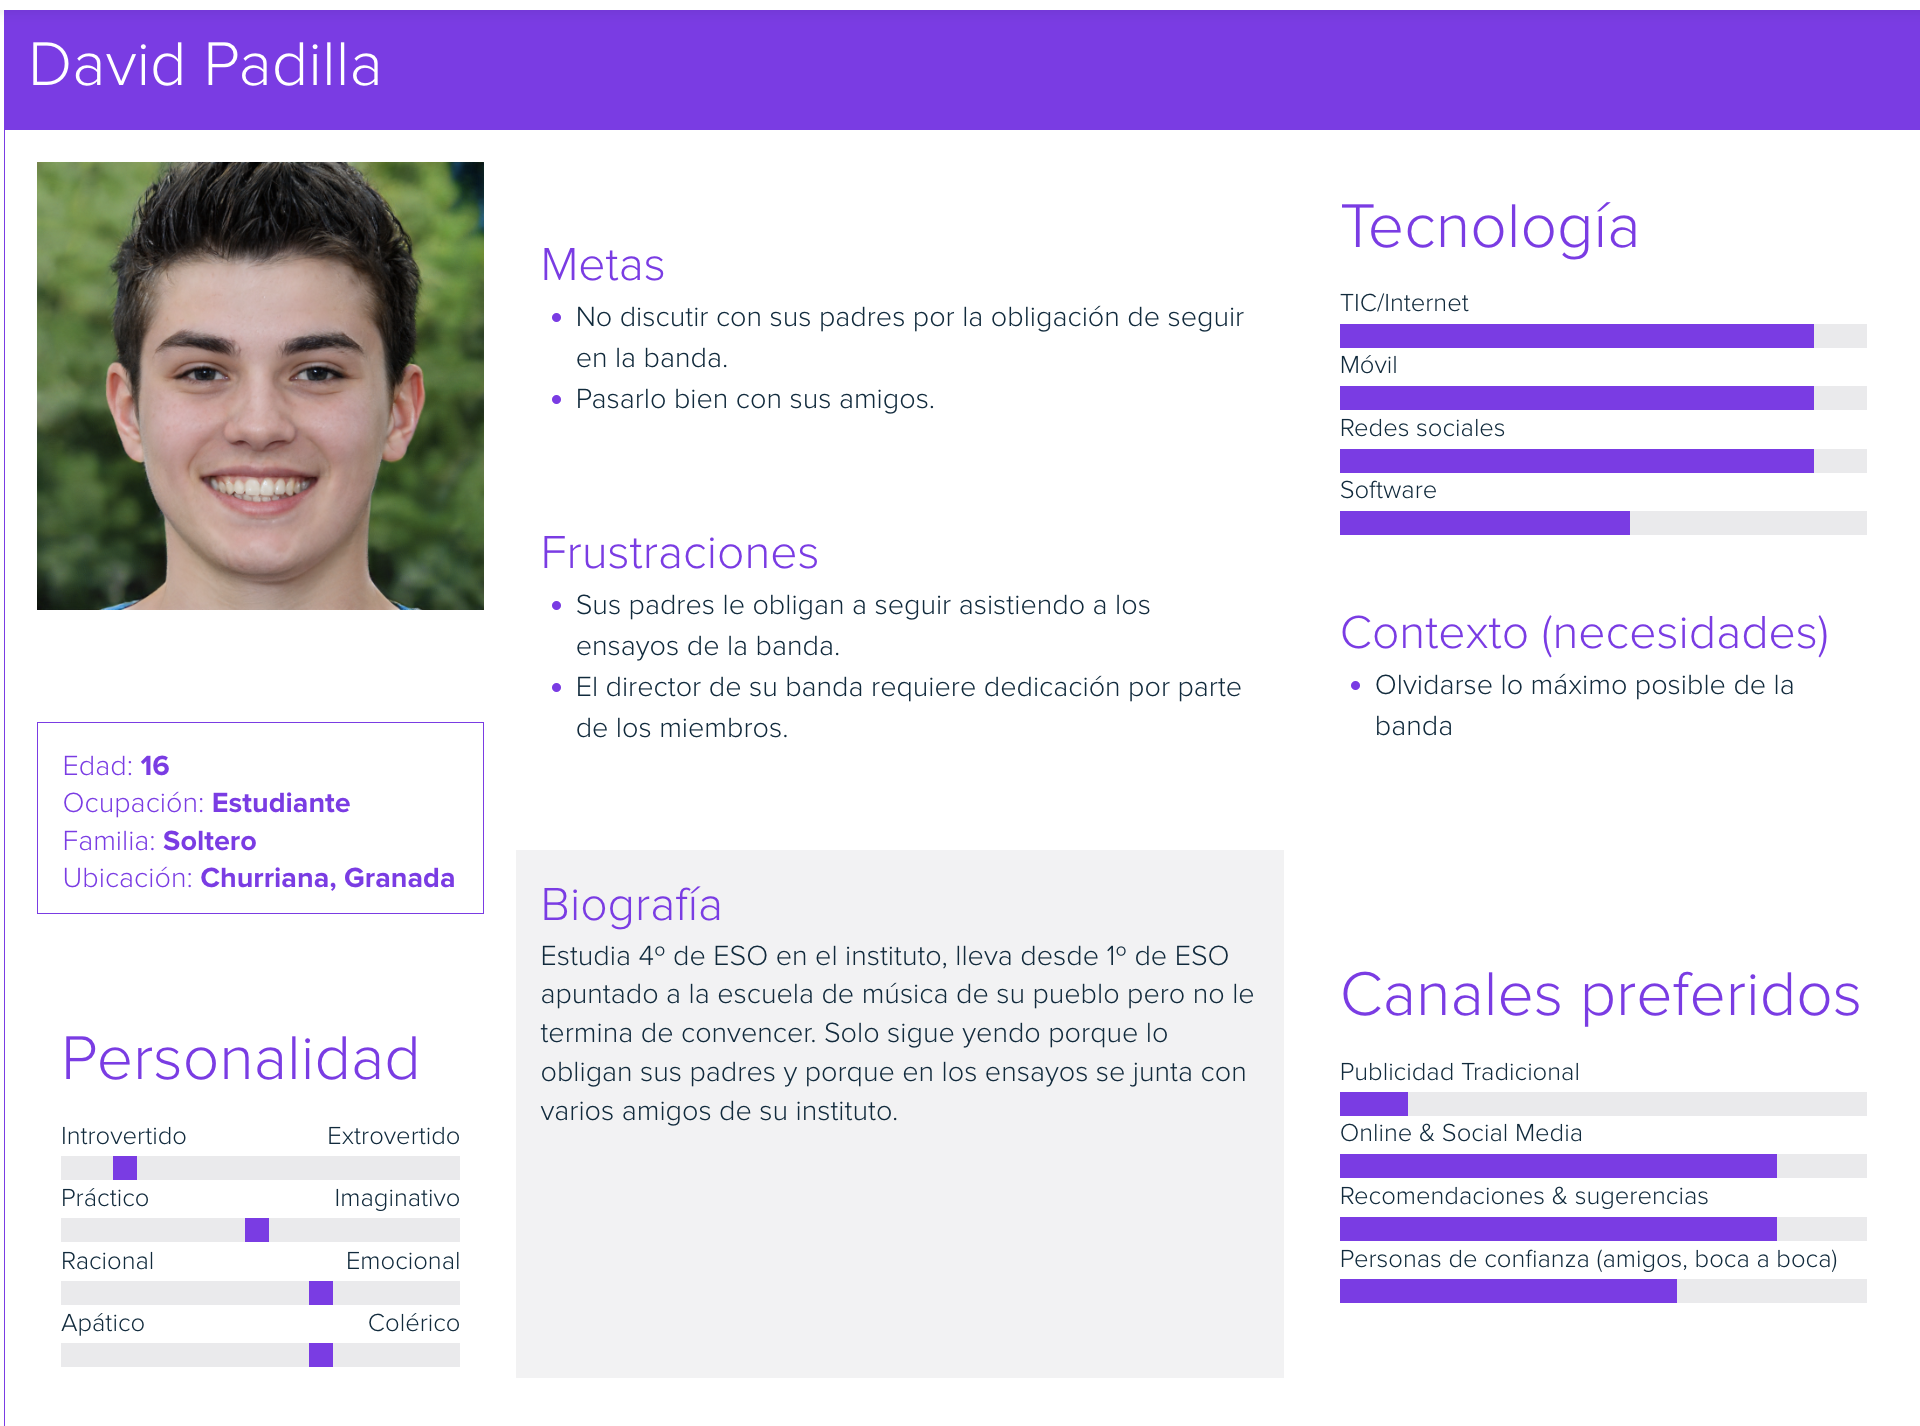
\includegraphics[width=0.8\textwidth]{imagenes/personas/persona_david.png}
\caption{Persona: Eugenio Soto}
\label{fig:persona_david}
\end{figure}

\begin{figure}[h]
\centering
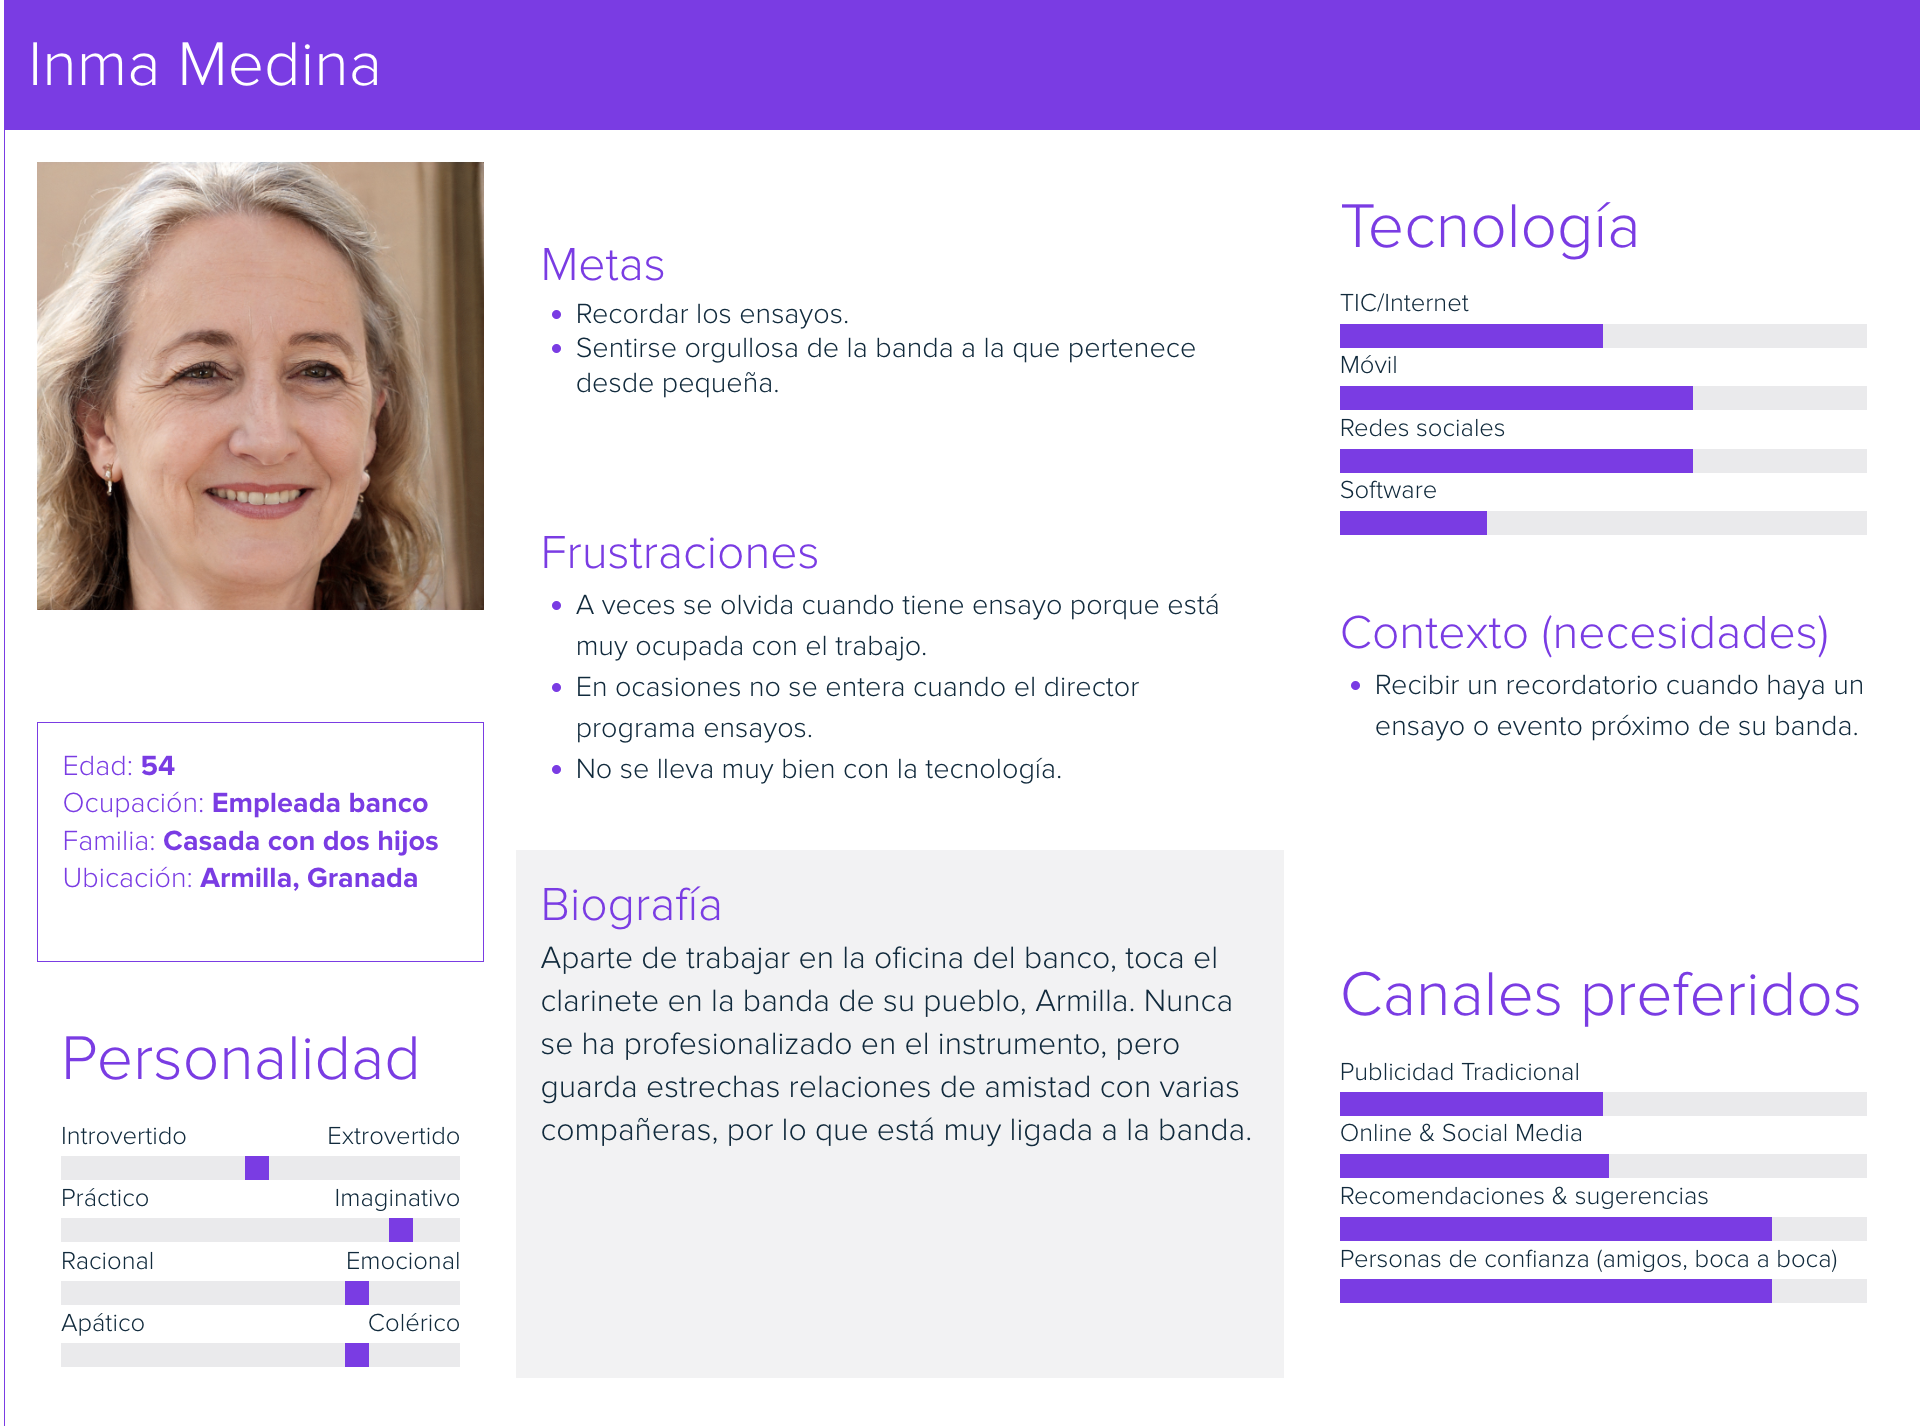
\includegraphics[width=0.8\textwidth]{imagenes/personas/persona_inma.png}
\caption{Persona: Inma Medina}
\label{fig:persona_inma}
\end{figure}

\section{Malla receptora de información}

La malla receptora de información (\textit{Feedback Capture Grid}) es un método para organizar feedback de manera estructurada en el cual se divide una hoja de papel en cuatro cuadrantes, cada uno representado con un símbolo diferente. El superior izquierdo se representa con un símbolo ``+'', y en él anota el feedback positivo. En el superior derecho, con símbolo de triángulo, se recogen las críticas. En el inferior izquierdo, con una interrogación, se añaden las preguntas que han surgido y en el inferior derecho, con una bombilla, las nuevas ideas que surgen.\cite{feedbackCaptureGrid}

A continuación se resumen los puntos recogidos para cada uno de los apartados.

\subsection{Aspectos interesantes o relevantes de la idea}

\begin{itemize}
    \item Está integrado en una app de mensajería.
    \item Funciona en todos los dispositivos móviles y de escritorio.
    \item El software es de código abierto.
    \item Lo puede utilizar cualquier agrupación.
    \item Se reciben notificaciones a través de la misma app de comunicación.
    \item Se pueden crear instancias del bot configurables a las necesidades de distintas agrupaciones.
\end{itemize}

\subsection{Críticas constructivas o posibilidades de mejora}

\begin{itemize}
    \item Depende del funcionamiento de Telegram.
    \item La interfaz es más limitada que una aplicación web.
    \item Se requiere tener cuenta de Telegram.
    \item Se requiere un servidor propio en el que esté alojada la aplicación para funcionar, o pagar el uso de uno en la nube.
    \item La interfaz en ordenador requiere de demasiados clics para llevar a cabo las tareas.
\end{itemize}

\subsection{Preguntas nuevas a partir de la experiencia del usuario}

\begin{itemize}
    \item ¿Cuál es el coste de mantener la aplicación?
    \item ¿Se podrá pedir algo al bot desde un grupo?
    \item ¿Se podrán elegir qué notificaciones y recordatorios queremos recibir?
    \item ¿Los administradores podrán ver informes de la asistencia a ensayos?
    \item ¿La aplicación fomentará la asistencia de los miembros a los ensayos?
    \item ¿Los usuarios más reacios a la tecnología sabrán usar el bot con soltura?
    \item ¿Se va a poder usar el bot en varios idiomas?
\end{itemize}

\subsection{Ideas que surgen}

\begin{itemize}
    \item Hacer también una aplicación web para no depender de Telegram.
    \item Implementar un sistema de premios para los usuarios que cumplan objetivos de asistencia.
    \item Tener una instancia del bot funcionando para las agrupaciones que no lo quieran tener en un servidor propio.
    \item Crear una página web con guías para el uso del bot.
    \item Implementar internacionalización con varios idiomas.
\end{itemize}

\section{Descripción de la propuesta}

Teniendo en cuenta el análisis que se ha hecho hasta ahora, se puede dar una propuesta de solución que responda a las preguntas y necesidades expuestas, tanto en las personas ficticias como en el \textit{Feedback Capture Grid}.

\subsection{Propuesta del producto}

Primeramente se determinan unas características y funcionalidades mínimas para tener un Producto Mínimo Viable, o MVP por sus siglas en inglés. El Producto Mínimo Viable es una técnica que se basa en disponer de suficientes características para satisfacer a los primeros usuarios, de manera que las siguientes funcionalidades se pueden desarrollar teniendo en cuenta el feedback de estos primeros usuarios.\cite{mvp} En nuestro caso, las funcionalidades incorporadas en esta primera versión serán:

\begin{enumerate}
    \item Agrupaciones:
    \begin{enumerate}
        \item {[Administrador]} Crear nuevas agrupaciones
        \item {[Administrador]} Eliminar agrupaciones
        \item {[Administrador]} Invitar miembros a la agrupación
        \item {[Administrador]} Eliminar miembros de la agrupación
        \item {[Usuario]} Unirse a una agrupación existente
        \item {[Usuario]} Salirse de una agrupación
        \item {[Usuario]} Ver todas las agrupaciones en las que estoy inscrito
        \item {[Usuario]} Ver el detalle de una agrupación
    \end{enumerate}
    \item Eventos:
    \begin{enumerate}
        \item {[Administrador]} Crear nuevos eventos en mi agrupación
        \item {[Administrador]} Eliminar eventos
        \item {[Administrador]} Invitar miembros a un evento
        \item {[Administrador]} Eliminar miembros de un evento
        \item {[Usuario]} Ver los eventos próximos
        \item {[Usuario]} Ver el detalle de un evento
    \end{enumerate}
    \item Asistencia:
    \begin{enumerate}
        \item {[Administrador]} Ver qué usuarios han respondido su asistencia a un evento
        \item {[Usuario]} Responder la asistencia a un evento
        \item {[Usuario]} Registrar la razón por la que no puedo asistir a un evento
    \end{enumerate}
    \item Recordatorios:
    \begin{enumerate}
        \item {[Usuario]} Recibir recordatorios diarios con los eventos de ese día
    \end{enumerate}
    \item Repertorio:
    \begin{enumerate}
        \item {[Administrador]} Añadir una obra a la agrupación
        \item {[Administrador]} Eliminar una obra la agrupación
        \item {[Administrador]} Subir partituras de las obras
        \item {[Administrador]} Eliminar una obra de la agrupación
        \item {[Usuario]} Ver las obras de mi agrupación
        \item {[Usuario]} Descargar las partituras de mi agrupación
    \end{enumerate}
    \item Administración:
    \begin{enumerate}
        \item {[Administrador]} Añadir administradores
        \item {[Administrador]} Quitar administradores
    \end{enumerate}
    \item Notificaciones:
    \begin{enumerate}
        \item {[Administrador]} Recibir notificación cuando un miembro responde sobre su asistencia
        \item {[Usuario]} Recibir notificación cuando se asigna un evento
    \end{enumerate}
\end{enumerate}


\subsection{Elección de metodología de desarrollo}

Dadas las características del proyecto, se va a apostar por una metodología de desarrollo ágil como es SCRUM, aunque con ciertas adaptaciones ya que el equipo de desarrollo va a estar compuesto por una sola persona.

Esta metodología ágil nos permitirá ir mejorando el producto a lo largo del desarrollo, pudiendo probarlo desde etapas tempranas. SCRUM es un método de desarrollo e innovación que enfatiza un conjunto de valores y prácticas para la gestión de proyectos, más que tratar requerimientos e implementación. Trata de hacer el proceso de la gestión más \textbf{empírico} que \textbf{definido}.\cite{scrum}

La naturaleza flexible del marco de trabajo SCRUM se adapta a proyectos como el que nos ocupa, dado que no se conocen todos los requisitos concretamente con antelación y nos ayuda a que el usuario sea parte del desarrollo, algo útil si queremos hacer un desarrollo centrado en el usuario.

\subsection{Planificación}

Para poder tener un producto que cumpla con los objetivos reseñados anteriormente, es necesario establecer en qué orden se van a realizar las distintas tareas.


\subsubsection{Planificación en sprints}

Dado que la metodología de desarrollo a usar será SCRUM, para la planificación del proyecto se va a usar uno de sus elementos más importantes como es la planificación de los sprints. 

Los sprints son eventos de una longitud fija, generalmente menor a un mes. Durante un sprint se intenta realizar todo el trabajo necesario para alcanzar el objetivo del producto.

Los sprints corresponden a objetivos concretos del producto, por lo que el resto de tareas (como la toma de decisiones o el aprendizaje) se van a incluir en la planificación temporal pero no como sprints. Los sprints planificados para este proyecto son:

\begin{enumerate}

\item \textbf{Primer sprint:} Se va a implementar un bot de prueba con funcionalidad de actualización de una base de datos de palabras. Este bot servirá como exploración de las distintas funcionalidades que se usarán posteriormente.
\item \textbf{Segundo sprint:} Se va a implementar la lógica para responder a los comandos de los usuarios, así como la funcionalidad para crear agrupaciones y unirse a una agrupación.
\item \textbf{Tercer sprint:} Se van a crear diversos plugins, uno para permitir guardar la sesión del usuario en la base de datos y otro para usar un menú de calendario que sirva para fijar las fechas de eventos. Estos plugins serán publicados.
\item \textbf{Cuarto sprint:} Se añadirá la funcionalidad básica relacionada con los eventos, como la creación y eliminación. También permitir a un miembro salirse de una agrupación, así como habilitar enlaces de invitación.
\item \textbf{Quinto sprint:} Se podrán añadir y eliminar obras a las agrupaciones. Función de edición de agrupaciones, eventos y obras. 
\item \textbf{Sexto sprint:} Notificaciones de asignación de eventos y adición de miembros a las agrupaciones además de recordatorios de los eventos diarios.
\end{enumerate}

\subsubsection{Planificación temporal}

La planificación del desarrollo del bot en el tiempo se sucederá de la siguiente forma:

\begin{itemize}
    \item Primeramente se tomarán las decisiones oportunas sobre las herramientas a utilizar, requisitos concretos del software y análisis de la competencia.
    \item Después habrá un periodo de formación en las herramientas necesarias para el desarrollo de la aplicación. Esta formación también se extenderá a lo largo de todo el desarrollo.
    \item Los sprints de desarrollo vendrán tras el periodo inicial de formación.
    \item Finalmente tendremos un periodo de pruebas y de finalización de la memoria.
\end{itemize}

En la tabla \ref{tab:planificacionTemporal} se muestra el tiempo estimado que requerirá cada tarea del desarrollo. Dado que el tiempo requerido para cada crédito ECTS es de entre 25 y 30 horas y esta asignatura es de 12 créditos, hablaríamos de 300-360 horas, sin embargo el tiempo para el desarrollo se estima mayor por la formación previa requerida en las nuevas tecnologías utilizadas. 

Este exceso de tiempo no se estima perjudicial dada la naturaleza formativa de este trabajo, ya que los conocimientos adquiridos podrán seguir siendo utilizados posteriormente a la finalización.

\begin{table}[]
    \centering
    \begin{tabular}{|c|c|}
        \hline
        Toma de decisiones & 10 horas \\
        \hline
        Formación   & 100 horas \\
        \hline
        Implementación & 150 horas \\
        \hline
        Pruebas & 10 horas \\
        \hline
        Memoria & 150 horas \\
        \hline
        \hline
        Total & 420 horas \\
        \hline
    \end{tabular}
    \caption{Planificación temporal}
    \label{tab:planificacionTemporal}
\end{table}


\subsubsection{Diagrama de Gantt}

El diagrama de Gantt que se puede ver en la figura \ref{fig:gantt} se ha construido teniendo en cuenta que cada día se van a trabajar 2 horas, por lo tanto se van a trabajar 210 días, o lo que es lo mismo, 42 semanas.

Así mismo, no se concretan las fechas reales ya que pueden cambiar por factores externos durante el desarrollo del proyecto.

\begin{figure}[h]
\centering
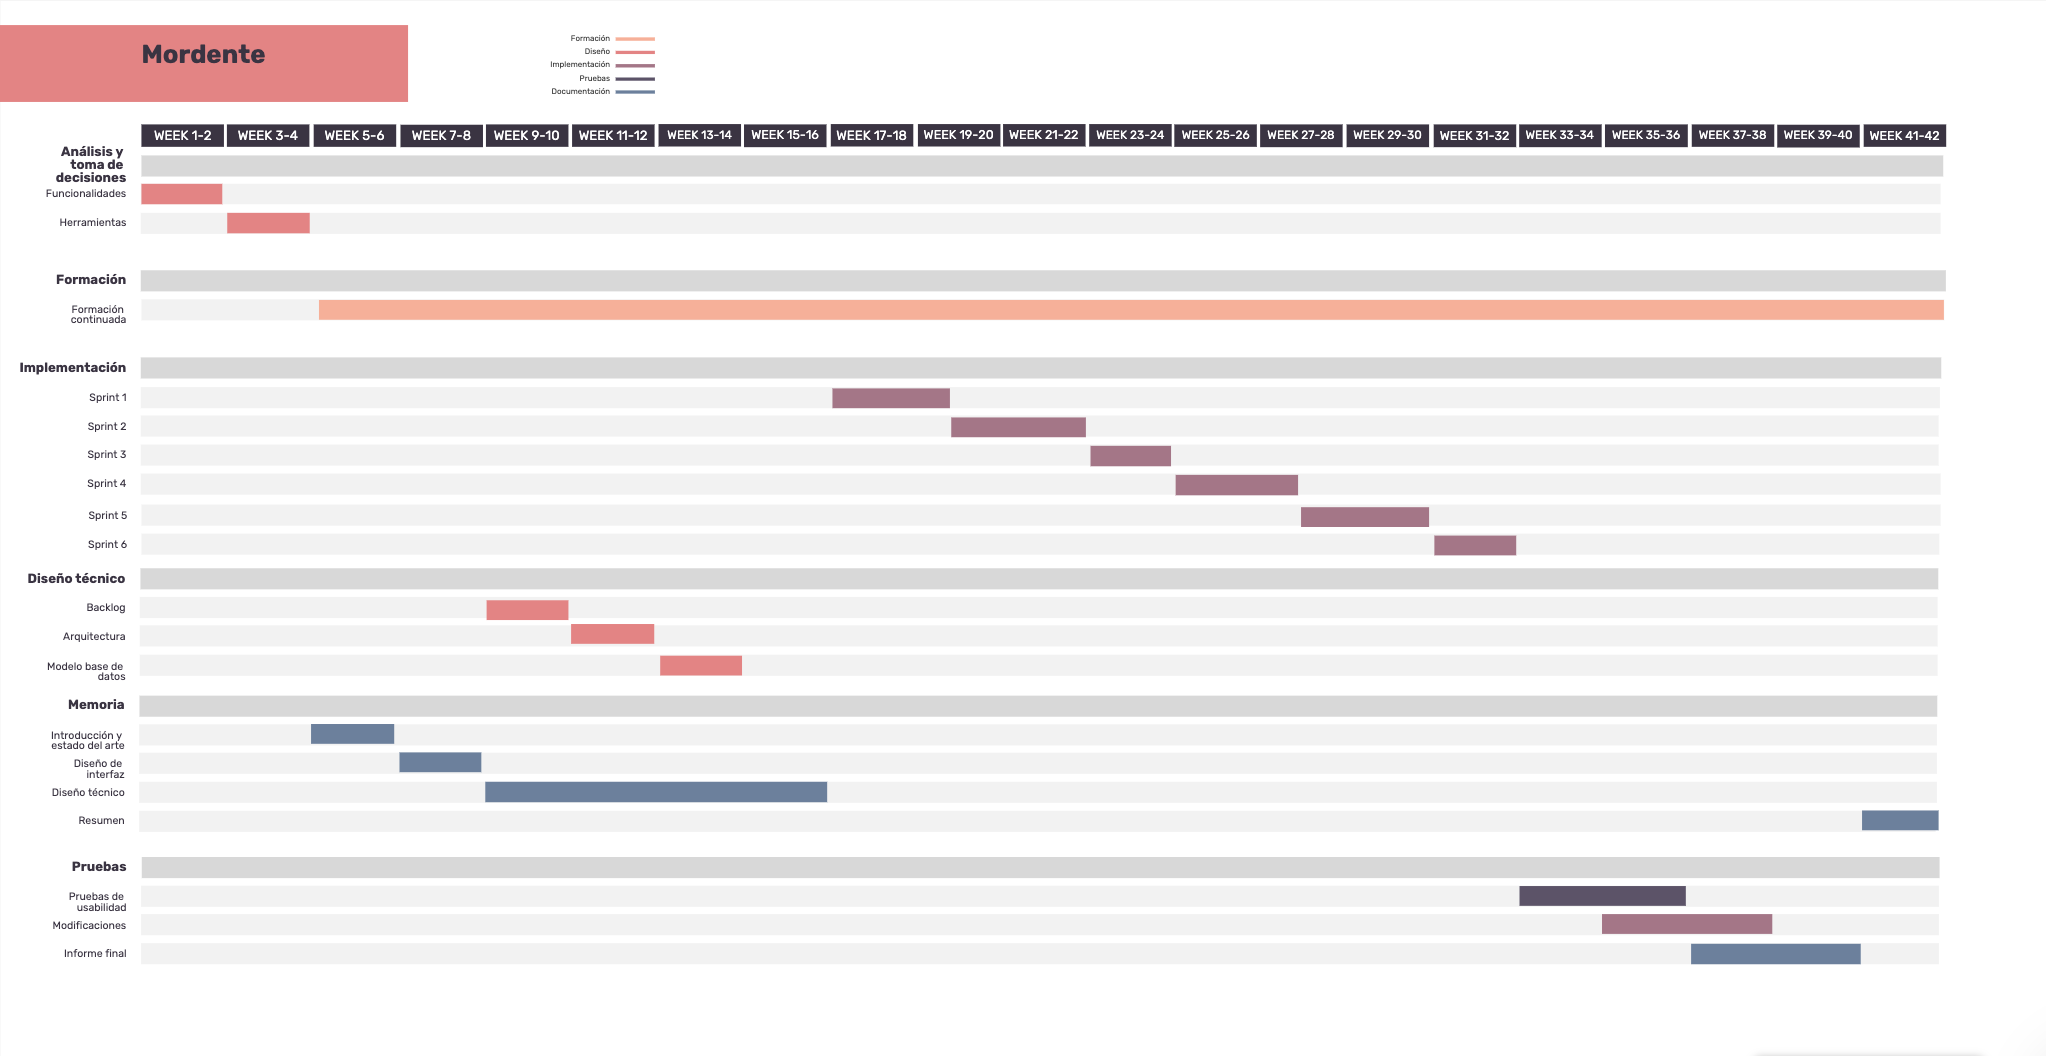
\includegraphics[angle=90,origin=c,width=0.85\textwidth]{imagenes/gantt.png}
\caption{Diagrama de Gantt del proyecto}
\label{fig:gantt}
\end{figure}


\subsection{Presupuesto}

El coste de infraestructura es nulo en esta primera versión, puesto que el bot puede estar alojado en un servidor propio o usando el plan gratuito de cualquier servicio de alojamiento de servidores virtuales en la nube. Por tanto, el coste a considerar es el del tiempo empleado por el desarrollador.

Según el Anexo I del XVII Convenio colectivo estatal de empresas de consultoría y estudios de mercado y de la opinión pública\footnote{\url{https://www.boe.es/diario_boe/txt.php?id=BOE-A-2018-3156}} el salario mínimo a partir del 31 de diciembre de 2019 para un Programador Junior es de 15860,56 euros al año. La tabla \ref{tab:presupuesto} muestra el presupuesto estimado teniendo en cuenta el siguiente cálculo y la suposición de 12 meses el año:


$$12\;\textnormal{meses} \times 4\;\frac{\textnormal{semanas}}{\textnormal{mes}} \times 40\;\frac{\textnormal{horas}}{\textnormal{semana}}  = 1920 {\textnormal{ horas}}$$

$${\textnormal{coste por hora: }} \frac{15860.56}{1920} = 8.26 {\textnormal{ \texteuro}}$$



\begin{table}[]
    \centering
    \begin{tabular}{|l|c|c|c|}
        \hline
        Concepto & Unidades & \texteuro/unidad & Total \\
        \hline
        Hora de Programador Junior & 420 & 8,26 & 3469,2 \\
        \hline
        \hline
        Total & & & 3469,2 \\
        \hline
    \end{tabular}
    \caption{Presupuesto}
    \label{tab:presupuesto}
\end{table}


